\section{Facit}

\setcounter{opgave}{0}

\begin{opgave}{Stirling}
    Lad os definere forholdet mellem Stirlings approksimation med hhv. 2 og 3 led.
    \[ S=\frac{N\ln(N)-N+\frac{1}{2}\ln(N)}{N\ln(N)-N} \]
    Så kan vi regne det for tilfældene:
    \begin{itemize}
        \item $N=10$. Her får vi $S\approx 1.088$.
        \item $N=100$. Her får vi $S\approx 1.0064$.
        \item $N=10^4$. Her får vi $S\approx 1.000056$.
        \item $N=N_A=6.022\times 10^{23}$. Her får vi $S\approx 1$ (det er lidt større end 1, men langt de fleste lommeregnere vil bare sige 1).
    \end{itemize}
    Fra ovenstående resultater ses, de to resultater bliver mere eller mindre ens, for store værdier af $N$.\\
    Igen kan vi definere forholdet mellem Stirlings approksimation med hhv. 1 og 2 led.
    \[ R=\frac{N\ln(N)}{N\ln(N)-N} \]
    Igen fås
    \begin{itemize}
        \item $N=10$. Her fås $R=1.77$.
        \item $N=100$. Her fås $R=1.28$.
        \item $N=10^4$. Her fås $R=1.12$.
        \item $N=N_A$. Her fås $R=1.019$.
    \end{itemize}
    Igen ses at de to resultater bliver mere og mere ens, jo større $N$ bliver. Men selv for meget store $N$, f.eks. $N_A$, er der stadig en relativ betydningsfuld afvigelse.
\end{opgave}

\begin{opgave}{Konfigurationer}
    \opg Vi beregner den samlede energi for de forskellige systemer, og tjekker om det passer til at den skal give $U=7\varepsilon$.
    \begin{enumerate}[label=\alph*)]
        \item $U=6\cdot 0\varepsilon+2\cdot 1\varepsilon+1\cdot 5\varepsilon=7\varepsilon$. Så denne konfiguration er mulig.
        \item $U=8\cdot 0\varepsilon+1\cdot 7\varepsilon=7\varepsilon$. Så denne konfiguration er mulig.
        \item $U=4\cdot 0\varepsilon+3\cdot 1\varepsilon+1\cdot 2\varepsilon+1\cdot 3\varepsilon=8\varepsilon$. Fordi den samlede energi af denne konfiguration ikke er den samme som for systemet, er det ikke en mulig konfiguration.
        \item $U=5\cdot 0\varepsilon+1\cdot 1\varepsilon+3\cdot 2\varepsilon=7\varepsilon$. Så denne konfiguration er mulig.
    \end{enumerate}
    \[ \]
    \opg Der er i alt $N=9$ partikler. Der er 7 partikler i tilstand $0$, 1 partikel i tilstand $3$ og 1 partikel i tilstand $4$. Derved kan vi bruge formlen
    \[ \Omega_n=\frac{N!}{\prod_{j=0}^\infty n_j!}, \]
    hvor $n_0=7$, $n_3=1$ og $n_4=1$.
    \[ \Omega_n=\frac{9!}{7!\cdot 1!\cdot 1!}=72 \]
    så svaret er b).
    \opg Den eneste konfiguration som har en partikel i $j=7$ tilstanden, og som på samme tid overholder energibegrænsningen $U=7\varepsilon$ er
    \[ [8,0,0,0,0,0,0,1,0,\dots]. \]
    Sandsynligheden for at finde en partikel i $j=7$ er derfor
    \[ p=\frac{\Omega_n}{\Omega}, \]
    hvor
    \[ \Omega_n=\frac{9!}{8!\cdot 1!}=9 \]
    og $\Omega$ er antallet af mikrotilstande \emph{for alle} konfigurationer.
    \begin{table}[H]
        \centering
        \begin{tabular}{lr}
            Konfiguration & Multiplicitet \\ \hline
            $[8,0,0,0,0,0,0,1]$ & 9\\
            $[7,1,0,0,0,0,1]$ & 72\\
            $[7,0,1,0,0,1]$ & 72\\
            $[7,0,0,1,1]$ & 72\\
            $[6,2,0,0,0,1]$ & 252\\
            $[6,1,1,0,1]$ & 504\\
            $[6,0,2,1]$ & 252\\
            $[6,1,0,2]$ & 252\\
            $[5,3,0,0,1]$ & 504\\
            $[5,2,1,1]$ & 1512\\
            $[5,1,3]$ & 504\\
            $[4,4,0,1]$ & 630\\
            $[4,3,2]$ & 1260\\
            $[3,5,1]$ & 504\\
            $[2,7]$ & 36
        \end{tabular}
    \end{table}
    Summen over alle multipliciteter giver 6435 forskellige mulige mikrotilstande. 9 af disse vil have en partikel i $j=7$ tilstanden. Hvis vi bruger den mikrokanoniske ensemble, bliver sandsynligheden derved
    \[ p=\frac{9}{6435}\approx \SI{0.14}{\percent}. \]
    \opg Ligevægtskonfiguration er den mest sandsynlige konfiguration. På ovenstående tabel kan vi se, at konfigurationen $[5,2,1,1]$ har den største multiplicitet, nemlig 1512, så den må være ligevægtskonfigurationen. Ligeledes regnes sandsynligheden med den mikrokanoniske ensemble.
    \[ p_0=\frac{1512}{6435}\approx \SI{23.5}{\percent} \]
    \opg Den totale entropi af systemet er Boltzmann entropien
    \[ S_B=k_B\ln(\Omega), \]
    hvor $\Omega$ er det totale antal mulige mikrotilstande. Så
    \[ S_B=k_B\ln(6435)=8.77k_B. \]
    \opg Vi regner entropien på samme måde, men hvor vi kun bruger multipliciteten for ligevægtskonfigurationen
    \[ S_{B,0}=k_B\ln(1512)=7.32k_B. \]
\end{opgave}

\begin{opgave}{Spillekort}
    \opg Hver mikrotilstand af en blandet bunke kort er en unik rækkefølge af kort i bunken. Hvis vi trækker det første kort fra bunken er der 52 forskellige muligheder. Dernæst er der 51 muligheder osv. Fortsætter vi dette, må det betyde at der er 
    \[ \Omega=52\cdot 51\cdot 50\cdot \cdots\cdot 2\cdot 1=52!\approx 8.07\cdot 10^{67} \]
    forskellige mikrotilstande.
    \opg (i) Hvis kulørerne er forskellige, har vi præcist den samme opgave som i første del, bare med 26 forskellige kort i stedet for 52. Multipliciteten er derfor
    \[ \Omega=26!\approx 4.03\cdot 10^{26}. \]
    (ii) Hvis kulørerne er ens, må det betyde at der findes to ens mikrotilstande for hver af de 13 kort. F.eks., hvis vi trækker begge $4\spadesuit$ som de første to kort. Enten kan vi trække $4\spadesuit$ fra det første sæt først, ellers trækker vi den anden $4\spadesuit$ først. Men i virkeligheden er dette den sammen mikrotilstand, fordi vi ikke kan kende forskel på kortene. For hvert kort er der altså \emph{halvt} så mange mikrotilstande som i del (i). Så
    \[ \Omega=\underbrace{\frac{26!}{2\cdot\cdots\cdot 2}}_{\text{13 gange}}=\frac{26!}{2^{13}}\approx 4.92\cdot 10^{22}. \]
    \opg Der er to kopier af 52 unikke kort, hvilket vil sige at der i alt er 104 kort. Hvis alle kort var forskellige ville der være $104!$ mikrotilstande. Men fordi at der er to kopier af hvert kort fra hvert dæk, vil der være halvt så mange mikrotilstande for hvert kort (fordi, hvis vi bytter rundt på to ens kort i bunken, så får vi sammen mikrotilstand). Så
    \[ \Omega_T=\frac{104!}{2^{52}}. \]
\end{opgave}

\begin{opgave}{Boltzmannfordelingen}
    \opg Lad $N=n_1+n_2+n_3$. Så er
    \[ \Omega_n=\frac{N!}{n_1!\cdot n_2!\cdot n_3!}. \]
    \opg Først tager vi logaritmen af svaret fra 1).
    \begin{align*}
        \ln(\Omega_n)&=\ln\left(\frac{N!}{n_1!\cdot n_2!\cdot n_3!}\right)\\
        &=\ln(N!)-\ln(n_1!)-\ln(n_2!)-\ln(n_3!)
    \end{align*}
    Stirlings approksimation er 
    \[ \ln(n!)\approx n\ln(n)-n \]
    Vi kan bruge kædereglen og produktreglen til at finde ændringen i $\ln(n!)$. (Her kan $n$ være $n_1$, $n_2$ eller $n_3$. Husk at $N$ er konstant, så den ændrer sig ikke!)
    \begin{align*} 
        \delta \ln(n!)&\approx\delta(n\ln(n)-n)\\
        &=\delta(n\ln(n))-\delta n\\
        &=\ln(n)\delta n+n\delta(\ln(n))-\delta n\\
        &=\ln(n)\delta n+n\frac{1}{n}\delta n-\delta n\\
        &=\ln(n)\delta n
    \end{align*}
    Derfor må
    \begin{align*}
        \delta(\ln(\Omega_n))&=\cancelto{0}{\delta\ln(N!)}-\delta\ln(n_1!)-\delta\ln(n_2!)-\delta\ln(n_3!)\\
        &=-\ln(n_1)\delta n_1-\ln(n_2)\delta n_2-\ln(n_3)\delta n_3.
    \end{align*}
    \opg For at bevare antallet af partikler, så må det samlede antal partikler i den nye konfiguration stadig være $N$. Hvis den originale konfiguration er
    \[ [n_1,n_2,n_3], \]
    således at $n_1+n_2+n_3=N$, så er den nye konfiguration
    \[ [n_1+\delta n_1, n_2+\delta n_2, n_3+\delta n_3] \]
    også overholde det samlede antal partikler
    \[ n_1+\delta n_1 + n_2+\delta n_2+ n_3+\delta n_3=N. \]
    Men $n_1+n_2+n_3=N$, så hvis vi trækker $N$ fra på begge sider får vi
    \[ \delta n_1+\delta n_2+\delta n_3=0. \]
    Dette er betingelsen for konstant $N$. Den totale energi i den originale konfiguration er
    \[ n_1\varepsilon_1+n_2\varepsilon_2+n_3\varepsilon_3=U. \]
    Ligeledes skal den totale energi for den nye konfiguration også være U:
    \[ (n_1+\delta n_1)\varepsilon_1+(n_2+\delta n_2)\varepsilon_2+(n_3+\delta n_3)\varepsilon_3=0 \]
    Trækker vi $U$ fra på begge sider får vi
    \[ \delta n_1\varepsilon_1+\delta n_2\varepsilon_2+\delta n_3\varepsilon_3=0. \]
    Dette er betingelsen for energibevarelse.
    \opg I ligevægt er $\delta(\ln(\Omega_n))=0$, så
    \[ \ln(n_1)\delta n_1+\ln(n_2)\delta n_2+\ln(n_3)\delta n_3=0. \]
    Vi kan isolere for $\delta n_1$ i betingelsen for konstant antal partikler
    \[ \delta n_1=-\delta n_2-\delta n_3. \]
    Hvis vi indsætter dette i den første ligninger får vi
    \begin{align*}
        0&=\delta n_2\left(\ln(n_2)-\ln(n_1)\right)+\delta n_3\left(\ln(n_3)-\ln(n_1)\right)\\
        &=\delta n_2\ln\left(\frac{n_2}{n_1}\right)+\delta n_3\ln\left(\frac{n_3}{n_1}\right).
    \end{align*}
    Ligeledes, hvis vi indsætter dette i betingelsen for energibevarelse fås
    \[ \delta n_2(\varepsilon_2-\varepsilon_1)+\delta n_3(\varepsilon_3-\varepsilon_1)=0. \]
    Med lidt algebraisk gymnastik, er det muligt at eliminere $\delta n_2$ og $\delta n_3$ fra de to ovenstående ligninger, således at
    \[ \frac{1}{\varepsilon_2-\varepsilon_1}\ln\left(\frac{n_2}{n_1}\right)=\frac{1}{\varepsilon_3-\varepsilon_1}\ln\left(\frac{n_3}{n_1}\right). \]
    \opg Lad os sætte ovenstående ligning lig en arbitrær konstant $-\beta$. Da får vi to ligninger
    \[ \frac{1}{\varepsilon_2-\varepsilon_1}\ln\left(\frac{n_2}{n_1}\right)=-\beta\quad\text{og}\quad\frac{1}{\varepsilon_3-\varepsilon_1}\ln\left(\frac{n_3}{n_1}\right)=-\beta. \]
    Løser vi for brøkerne inde i logaritmerne, fås
    \[ \frac{n_3}{n_1}=e^{-\beta(\varepsilon_3-\varepsilon_1)}\quad\text{og}\quad\frac{n_2}{n_1}=e^{-\beta(\varepsilon_2-\varepsilon_1}. \]
\end{opgave}

\begin{opgave}{Adiabatisk ekspansion}
    \opg Sandsynligheden for at finde et molekyle i det originale volumen, afhænger naturligvis af både $V$ og $V_0$. Hvis $V$ er dobbelt så stort som $V_0$, så må der jo være en 50\% chance for at finde molekylet i det originale volumen, medens hvis den er fire gange så stor, giver det intuitivt mening af sandsynligheden må være 25\%. (Her skal man selvfølgelig antage, at molekylets placering er fuldkomment tilfældigt og ikke biased af andre molekyler) Vi finder frem til at 
    \[ p=\frac{V_0}{V}. \]
    \opg Chancen for at finde et molekyle i det originale volumen er $V_0/V$. Hvis molekylernes placering ikke afhænger af hinanden, må der være samme chance for alle $N$ molekyler. Så
    \[ p_0=\left(\frac{V_0}{V}\right)^N. \]
    \opg Hvis $\Omega_0$ er multipliciteten for systemet med alle molekyler i det originale volumen $V_0$, så må sandsynligheden $p_0$ for at finder molekylerne dér, være
    \[ p_0=\frac{\Omega_0}{\Omega}=\left(\frac{V_0}{V}\right)^N. \]
    Hvis vi løser ligningen for $\Omega$, får man
    \[ \Omega=\Omega_0\left(\frac{V}{V_0}\right)^N. \]
    \opg Ændringen i Boltzmann entropien, når man fjerner væggen er
    \begin{align*}
        \Delta S_B&=k_B\ln(\Omega)-k_B\ln(\Omega_0)\\
        &=k_B\ln\left(\frac{\Omega}{\Omega_0}\right)\\
        &=k_B\ln\left(\left(\frac{V}{V_0}\right)^N\right)\\
        &=Nk_B\ln\left(\frac{V}{V_0}\right).
    \end{align*}
\end{opgave}

\begin{opgave}{Exciteret konfiguration}
    \opg For at finde ligevægtskonfigurationen skal vi maksimere entropi (altså $\ln(\Omega_n)$) med hensyn til begrænsningen
    \[ \sum_{j=1}^Mn_j=N. \]
    Ligesom da vi maksimerede entropi for at komme frem til Boltzmannfordelingen, kan vi løse ved at skrive Lagrange multiplieren.
    \[ \frac{\partial}{\partial n_j}\left[\ln(\Omega_n)-\alpha\sum_i n_i\right]=0 \]
    Her er $\alpha$ er konstant og ligningen skal gælde for alle tilstande $j$. Dette giver
    \[ \frac{\partial}{\partial n_j}\left[\ln(\Omega_n)\right]-\alpha=0. \]
    Men
    \[ \Omega_n=\frac{N!}{\prod_j n_j!}, \]
    så
    \[ \Omega_n=\ln(N!)-\sum_j\ln(n_j!). \]
    Hvis vi benytter Stirlings approksimation på hvert led får vi
    \[ \Omega_n\approx N\ln(N)-N-\sum_j\left(n_j\ln(n_j)-n_j\right). \]
    Så
    \begin{align*}
        \frac{\partial}{\partial n_j}\left[\ln(\Omega_n)\right]&\approx\frac{\partial}{\partial n_j}\left[\cancelto{0}{N\ln(N)-N}-\sum_j\left(n_j\ln(n_j)-n_j\right)\right]\\
        &=-\frac{\partial}{\partial n_j}\left[ n_j\ln(n_j)-n_j\right]\\
        &=-\left[\ln(n_j)+\frac{n_j}{n_j}-1\right]\\
        &=-\ln(n_j).
    \end{align*}
    Derfor er
    \[ -\ln(n_j)-\alpha=0 \]
    for alle $j$. Løses for $n_j$ bliver det
    \[ n_j=e^\alpha. \]
    Bemærk at $\alpha$ er en konstant, så alle $n_j$ må være konstant (og ens!). Med andre ord bliver summen
    \[ \sum_{j=1}^M n_j=Mn_j=N. \]
    Løses for $n_j$ giver det
    \[ n_j=\frac{N}{M}. \]
    Dette svarer lige præcis til, at de $N$ partikler bliver fordelt mellem de $M$ kasser.
    \opg Sandsynligheden for ligevægtskonfigurationen er
    \[ p_0=\frac{\Omega_0}{\Omega}, \]
    hvor $\Omega_0$ er multipliciteten for ligevægtskonfigurationen og $\Omega$ er multipliciteten over alle konfigurationer. Hver af de $N$ partikler kan placeres i en af de $M$ kasser. Så antallet af forskellige mulige måde at arrangere systemet er
    \[ \Omega=M^N. \]
    Multipliciteten for ligevægtskonfigurationen er
    \[ \Omega_0=\frac{N!}{\prod_{j=1}^M n_j!}=\frac{N!}{\left(\left(\frac{N}{M}\right)!\right)^M}. \]
    Så
    \[ p_0=\frac{N!}{M^N}\left(\left(\frac{N}{M}\right)!\right)^{-M}. \]
    \opg Taylorudvidelsen for Stirling approksimationen er
    \[ \ln(n!)\approx\underbrace{\ln(n_0!)}_{\text{0. orden, $f(n_0)$.}}+\underbrace{\ln(n_0)\delta n}_{\text{1. orden, $f'(n_0)\delta n$}}+\underbrace{\frac{\delta n^2}{2n_0}}_{\text{2. orden, $\frac{1}{2}f''(n_0)\delta n^2$}}. \]
    Nu kan vi beregne ændringen $\ln(\Omega_n)$ når vi ændrer på antallet af partikler i én kasse med $\delta n$.
    \begin{align*}
        \delta\left(\ln(\Omega_n)\right)&\approx -\ln\underbrace{\left((n_0+\delta n)!\right)}_{\text{$n!$}}+\ln\left(n_0!\right)\\
        &=\cancel{-\ln(n_0!)}-\ln(n_0)\delta n-\frac{\delta n^2}{2n_0}+\cancel{\ln(n_0!)}\\
        &=-\ln(n_0)\delta n-\frac{\delta n^2}{2n_0}.
    \end{align*}
    Men der er \underline{to kasser}, hver med en ændring på hhv. $+\delta n$ og $-\delta n$. Derfor bliver den samlede ændring
    \begin{align*}
        \delta\left(\ln(\Omega_n)\right)&\approx\cancel{-\ln(n_0)(+\delta n)}-\frac{\delta n^2}{2n_0}-\cancel{\ln(n_0)(-\delta n)}-\frac{\delta n^2}{2n_0}\\
        &=-\frac{\delta n^2}{n_0}
    \end{align*}
    Derfra får man at
    \[ \delta\left(\ln(\Omega_n)\right)=\ln(\Omega_n)-\ln(\Omega_0)\approx -\frac{\delta n^2}{n_0} \]
    så
    \[ \ln(\Omega_n)\approx \ln(\Omega_0)-\frac{\delta n^2}{n_0}. \]
    \opg Først løses for $\Omega_n$:
    \begin{align*}
        \Omega_n&=e^{\ln(\Omega_0)-\frac{\delta n^2}{n_0}}\\
        &=\Omega_0 e^{-\frac{\delta n^2}{n_0}}
    \end{align*}
    Sandsynligheden for at få den nye konfiguration er
    \begin{align*} 
        p_n&=\frac{\Omega_n}{\Omega}\\
        &=\frac{1}{\Omega}\Omega_0e^{-\frac{\delta n^2}{n_0}}\\
        &=\left(\frac{\Omega_0}{\Omega}\right)e^{-\frac{\delta n^2}{n_0}}\\
        &=p_0e^{-\frac{\delta n^2}{n_0}}.
    \end{align*}
    \opg Med samme fremgangsmåde får vi
    \begin{align*}
        \delta\left(\ln(\Omega_n)\right)&\approx\sum_j\left[-\ln(n_0)\delta n_j-\frac{\delta n_j^2}{2n_0}\right]\\
        &=-\ln(n_0)\left[\sum_j\delta n_j\right]-\sum_j\frac{\delta n_j^2}{2n_0}.
    \end{align*}
    Men antallet af partikler skal være bevaret, så hvis man adderer ændringen i alle kasser samlet, skal det give nul.
    \[ \sum_j \delta n_j=0 \]
    Så
    \[ \delta\left(\ln\left(\Omega_n\right)\right)=\ln(\Omega_n)-\ln(\Omega_0)\approx -\sum_j\frac{\delta n_j^2}{2n_0}. \]
    Nu løses for $\ln(\Omega_n)$.
    \[ \ln(\Omega_n)\approx \ln(\Omega_0)-\sum_j\frac{\delta n_j^2}{2n_0} \]
    \opg Igen isolerer man først for $\Omega_n$ og indsætter beregner
    \begin{align*}
        p_n&=\frac{\Omega_n}{\Omega}\\
        &=\frac{\Omega_0}{\Omega}e^{-\sum_j\frac{\delta n^2_j}{2n_0}}\\
        &=p_0e^{-\sum_j\frac{\delta n^2_j}{2n_0}}.
    \end{align*}
    \opg For et stort antal kasser kan man antage, at ændringerne er uafhængige af hinanden. Sandsynligheden for at få ligevægtskonfigurationen kan vi derfor approksimere til at være
    \[ p_0\approx p_{n_0}^M, \]
    hvor $p_{n_0}$ er sandsynligheden for at der er $n_0$ partikler i kassen. Bemærk at sandsynligheden for at få konfigurationen
    \[ [n_0+\delta n_1, n_0+\delta n_2,\dots,n_0+\delta n_M] \]
    som blev udledt i delopgave 6) kan skrives som
    \[ p\approx p_{n_0}^Me^{-\sum_j\frac{\delta n^2_j}{2n_0}}=\prod_{j=1}^M \left[p_{n_0}e^{-\frac{\delta n^2_j}{2n_0}}\right]. \]
    Dette er altså sandsynligheden for at have $n_0+\delta n_1$ partikler i den første kasse, ganget sandsynligheden for at have $n_0+\delta n_2$ partikler i den anden kasse osv. Sandsynligheden for at have $n_0+\delta n_j$ partikler i den $j$'te kasse må derfor være et enkelt led
    \[ p\approx p_{n_0}e^{-\frac{\delta n_j^2}{2n_0}}. \]
\end{opgave}

\begin{opgave}{Paramagnetisme}
    \opg Tilstandssummen er
    \[ Z_1=e^{-\beta\varepsilon_0}+e^{-\beta\varepsilon_1}. \]
    \opg Vi laver et lille trick, hvor vi plusser med nul,
    \begin{align*}
        Z_1&=e^{-\beta\varepsilon_0}+e^{-\beta(\varepsilon_1-\varepsilon_0)-\beta\varepsilon_0}\\
        &=e^{-\beta\varepsilon_0}+e^{-\beta\varepsilon_0}e^{-\beta(\varepsilon_1-\varepsilon_0)}\\
        &=e^{-\beta\varepsilon_0}\left(1+e^{-\beta\varepsilon}\right).
    \end{align*}
    \opg Sandsynligheden for hhv. at være i grundtilstanden med energi $\varepsilon_0$ og den første exciterede tilstand med energi $\varepsilon_1$ er
    \[ p_0=\frac{1}{Z_1}e^{-\beta\varepsilon_0}\quad\text{og}\quad p_1=\frac{1}{Z_1}e^{-\beta\varepsilon_1}. \]
    Antallet af optagede tilstande er $n_0=Np_0$ og $n_1=Np_1$. For $n_0$ giver dette
    \[ n_0=\frac{Ne^{-\beta\varepsilon_0}}{e^{-\beta\varepsilon_0}\left(1+e^{-\beta\varepsilon}\right)}=\frac{N}{1+e^{-\beta\varepsilon}}. \]
    Og for $n_1$,
    \[ n_1=\frac{Ne^{-\beta\varepsilon_1}}{e^{-\beta\varepsilon_0}\left(1+e^{-\beta\varepsilon}\right)}=\frac{Ne^{-\beta\varepsilon}}{1+e^{-\beta\varepsilon}}. \]
    Hvis man er i tvivl om resultatet er sandt, kan man altid tjekke om $n_0+n_1=N$.
    \opg Bemærk at $\beta\varepsilon=\varepsilon/k_BT=\theta/k_B$. Hvis vi erstatter dette i $Z_1$ giver det
    \[ Z_1=e^{-\beta\varepsilon_0}\left(1+e^{-\theta/T}\right). \]
    Ligeledes for $n_0$ og $n_1$ giver det
    \[ n_0=\frac{N}{1+e^{-\theta/T}} \]
    \[ n_1=\frac{Ne^{-\theta/T}}{1+e^{-\theta/T}} \]
    \opg 
    \begin{figure}[H]
        \centering
        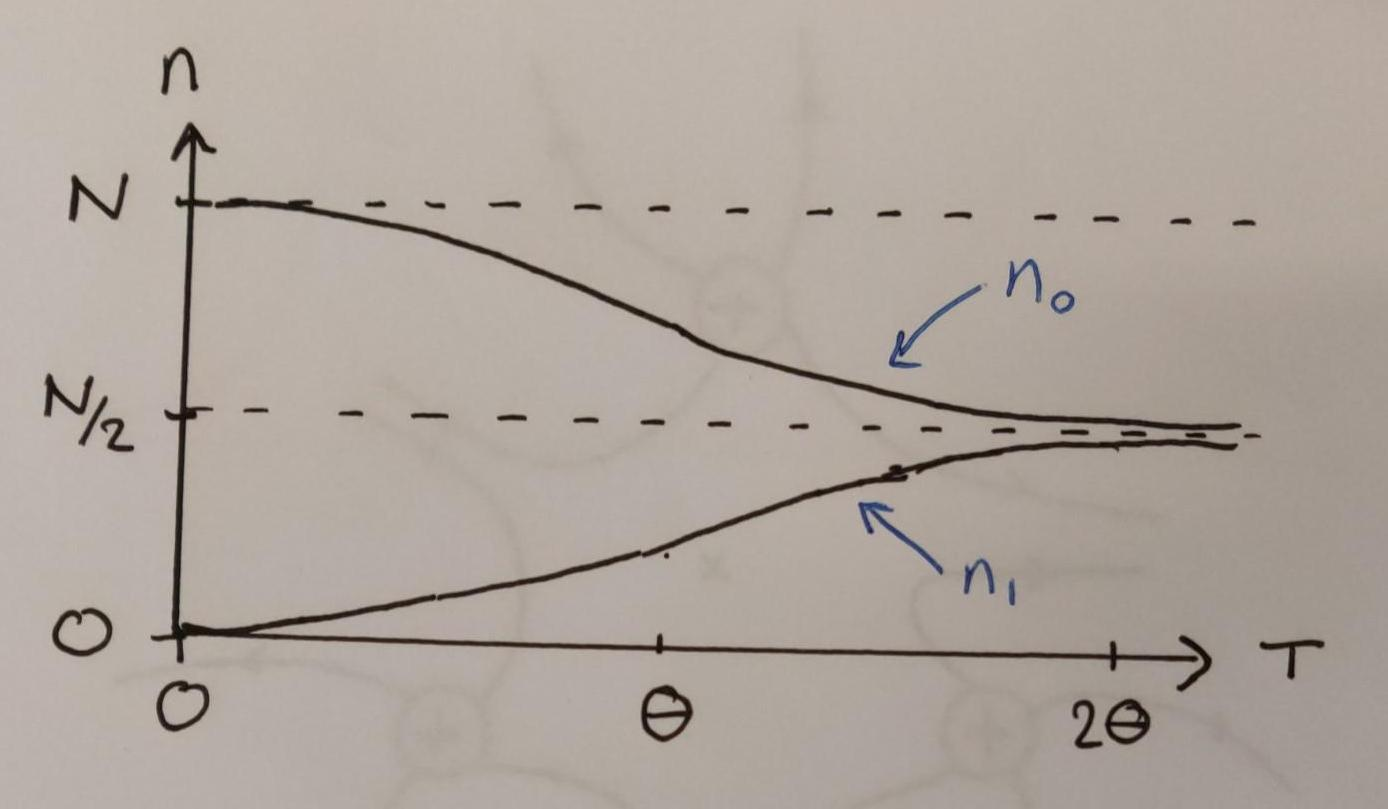
\includegraphics[width=0.8\textwidth]{facit/figurer/statfys/statfys_opg7,5.jpg}
    \end{figure}
    For $T\to 0$: $n_0=1$ og $n_1=0$.\\
    For $T\to\infty$: $n_0=n_1=N/2$.
    \opg Energiforskellen mellem de to energiniveauer er
    \[ \varepsilon=\varepsilon_1-\varepsilon_0=\mu B-(-\mu B)=2\mu B. \]
    Indsætter vi dette i vores ligninger får man
    \[ n_0=\frac{N}{1+e^{-2\beta\mu B}} \]
    \[ n_1=\frac{Ne^{-2\beta\mu B}}{1+e^{-2\beta\mu B}}. \]
    Magnetiseringen er
    \begin{align*}
        M&= n_0\mu-n_1\mu\\
        &=N\mu\left(\frac{1-e^{-2\beta\mu B}}{1+e^{-2\beta\mu B}}\right)\\
        &=N\mu\left(\frac{e^{\beta\mu B}-e^{-\beta\mu B}}{e^{\beta\mu B}+e^{-\beta\mu B}}\right)\\
        &=N\mu\tanh(\beta\mu B)\\
        &=N\mu\tanh\left(\frac{\mu B}{k_BT}\right)
    \end{align*}
    \opg
    \begin{figure}[H]
        \centering
        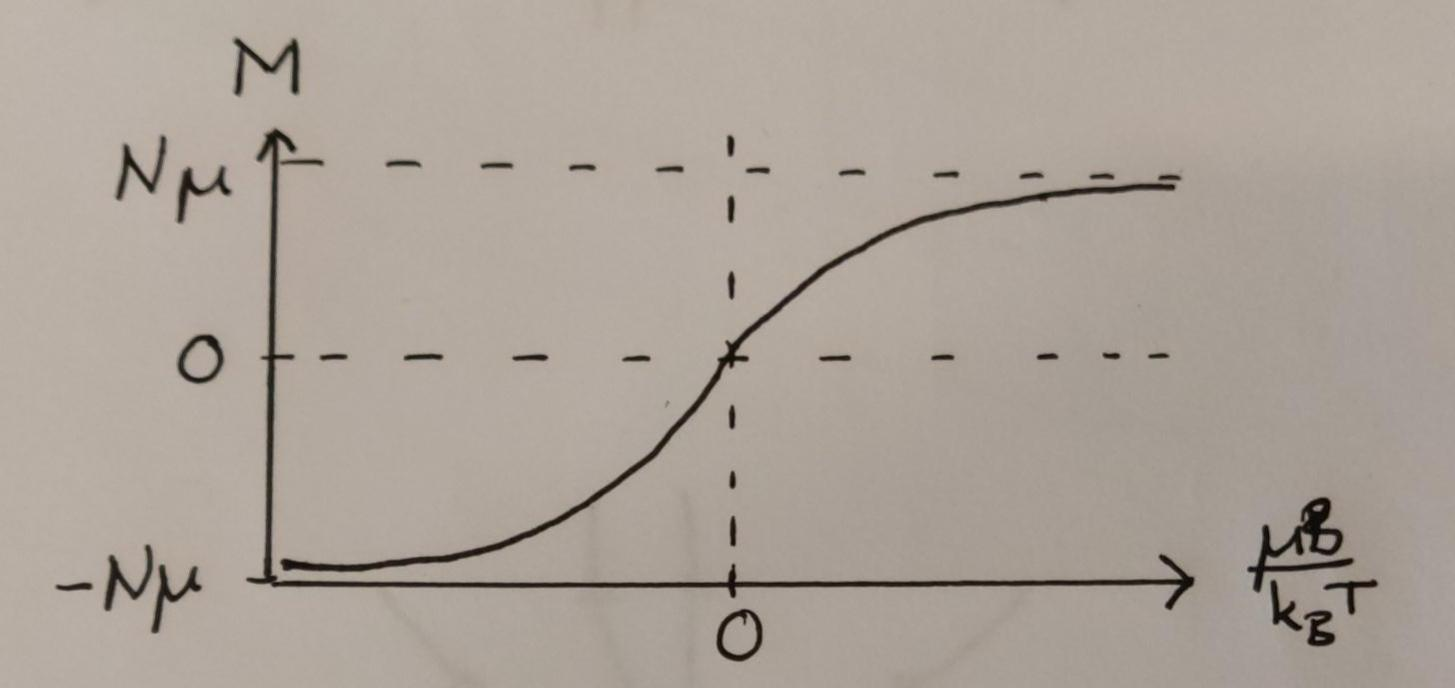
\includegraphics[width=0.8\textwidth]{facit/figurer/statfys/statfys_opg7,7.jpg}
    \end{figure}
    Det vil sige at for et meget stærkt magnetisk felt $B$, vil flere og flere dipoler orientere sig i samme retning som feltet. Hvis vi øger temperaturen, bliver færre dipoler magnetiseret (tilfældig orientering ved $T\to\infty$).
    \opg Bemærk at
    \[ \theta=\varepsilon/k_B=\frac{2\mu B}{k_B}, \]
    så for $\frac{2\mu B}{k_B}\ll T$, så må $\tanh\left(\frac{\mu B}{k_BT}\right)$ være meget lille. Vi kan derfor approksimere
    \[ M\approx N\mu\frac{\mu B}{k_BT}. \]
    Løses for $M/B$ ses
    \[ \frac{M}{B}\approx\frac{1}{T}\frac{N\mu^2}{k_B}. \]
    Dermed er der vist en proportionalitet mellem $M/B$ og $1/T$. Dette er Curies lov.
    \opg Hvis partiklernes orientering ikke kan justeres med hensyn til feltet, må magnetiseringen $M$ være konstant. Når vi gør $B$ lille
    \[ \frac{M}{B}\propto\frac{1}{T}\]
    kan vi se at temperaturen $T$ også skal blive mindre. Systemet bliver derfor koldere, når vi langsomt gør magnetfeltets styrke svagere!
    \opg Hvis magnetfeltets retning peget modsat i forhold til retningen af dipolerne, får det et negativt fortegn. Det vil sige at $M/B$ er negativ, så den eneste måde det kan give mening, er hvis temperaturen også er negativ!\\
    Selvom dette virker meget kontraintuitivt, er negativ temperatur noget som man ofte bruger inden for f.eks. statistisk fysik og laser fysik. Hvis du er interesseret, læs evt. om ``population inversion'' i lasere.
\end{opgave}

\begin{opgave}{Elastik}
    \opg Lad os sætte loddets potentielle energi til at være nul, når den er i vandret højde. Hvis et segment peger opad, vil loddet være i en højde $+a$. Hvis segmentet peger ned, vil loddet være i en højde $-a$. Derfor giver det mening at sætte $\varepsilon_\downarrow=-mga$ og $\varepsilon_\uparrow=+mga$. Derfra kan vi skrive tilstandssummen
    \[ Z=e^{-\beta\varepsilon_\downarrow}+e^{-\beta\varepsilon_\uparrow}=e^{\beta mga}+e^{-\beta mga}. \]
    Sandsynligheden for at segmentet peger op eller ned er
    \[ p_\downarrow=\frac{e^{\beta mga}}{e^{\beta mga}+e^{-\beta mga}} \]
    og
    \[ p_\uparrow=\frac{e^{-\beta mga}}{e^{\beta mga}+e^{-\beta mga}}. \]
    (Bemærk, at hvis tyngdekraften peger nedad, så $g>0$, og temperaturen er større end nul, $\beta>0$, så er $\beta mga>0$. Det betyder at der er større chance for at loddet hænger nedad end opad)
    \opg Ændringen i loddets potentielle energi bliver $\Delta\varepsilon=-2mga$. Det må betyde, at loddet kan befinde sig i højder
    \[ h=-Na,-(N-2)a,\dots,-2a,0,2a,\dots,(N-2)a,Na. \]
    Så tilstandssummen bliver
    \[ Z=e^{-\beta mgaN}+e^{-\beta mga(N-2)}+\cdots+e^{-2\beta mga}+1+e^{2\beta mga}+\cdots+e^{\beta mga(N-2)}+e^{\beta mgaN}. \]
    Hvis man sammensætter alle eksponentielfunktionerne i par $e^{x}+e^{-x}$, kan vi bruge identiteten
    \[ 2\cosh(x)=e^{x}+e^{-x}. \]
    Tilstandssummen bliver
    \[ Z=1+2\cosh(2\beta mga)+2\cosh\left(4\beta mga\right)+\cdots +2\cosh\left(N\beta mga\right). \]
    \opg Antag, at positiv længde er nedad. Så kan længden skrives som
    \begin{align*}
        L&=Nap_\downarrow-Nap_\uparrow\\
        &=Na\left(\frac{e^{\beta mga}-e^{-\beta mga}}{e^{\beta mga}+e^{-\beta mga}}\right)\\
        &=Na\tanh\left(\frac{mga}{k_BT}\right)
    \end{align*}
    \opg Når vi varmer på elastikken, gør vi $T$ større. Således bliver brøken $\frac{mga}{k_BT}$ mindre, så $\tanh$ funktionen bliver også mindre. Derfor må $L$ blive mindre.\\
    Elastikken bliver derfor kortere, når man varmer på den.
\end{opgave}